\begin{figure}[h!]
   \centering
   \begin{subfigure}[b]{0.4\textwidth}
      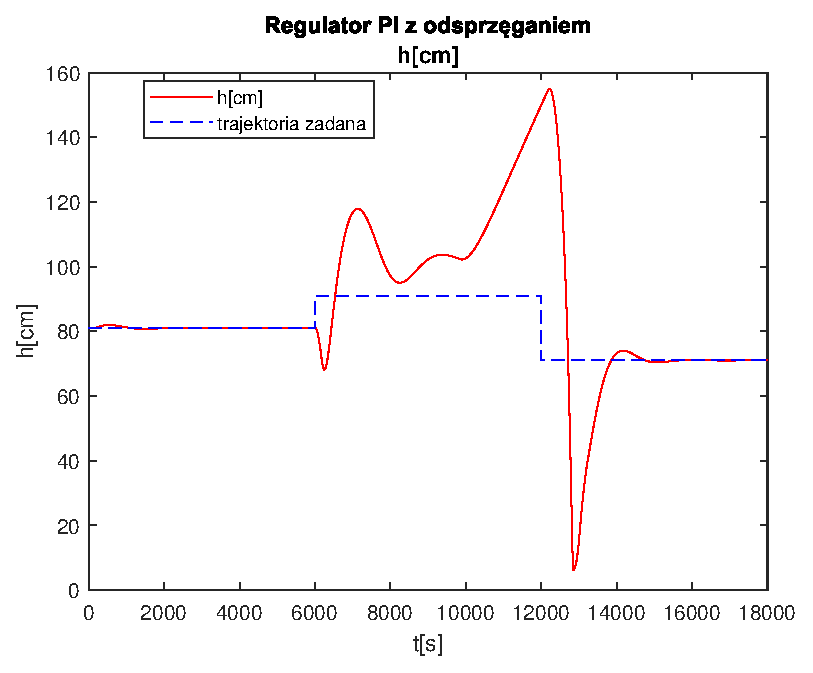
\includegraphics[width=1\linewidth]{img/PI/decoupler/noDisturbance/PIDecouplerH1Linfalse.eps}
      \caption{}
      \label{fig:fig:PIDecoupler1Linfalse1}
   \end{subfigure}
       
   \begin{subfigure}[b]{0.4\textwidth}
      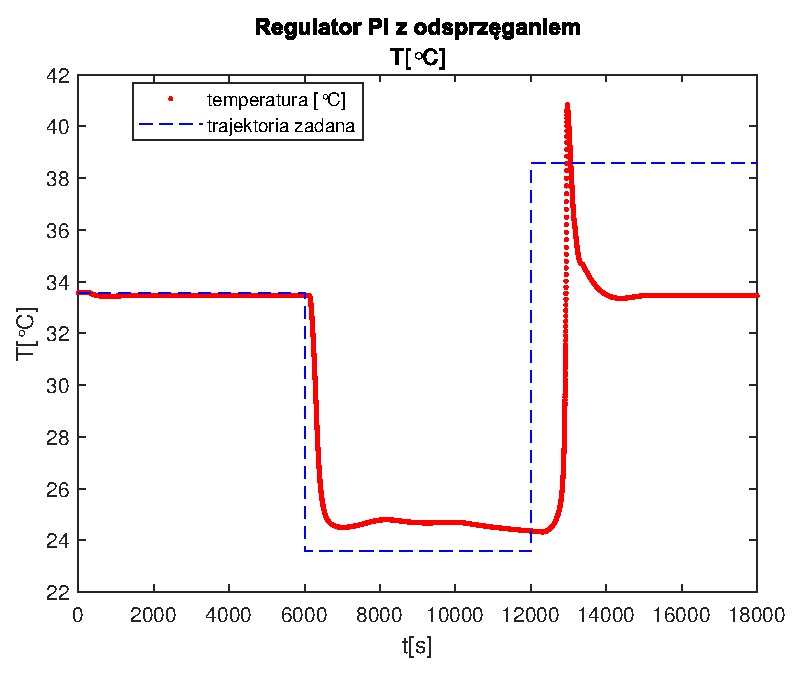
\includegraphics[width=1\linewidth]{img/PI/decoupler/noDisturbance/PIDecouplerT1Linfalse.eps}
      \caption{}
      \label{fig:fig:PIDecoupler1Linfalse2}
   \end{subfigure}
       
   \begin{subfigure}[b]{0.4\textwidth}
      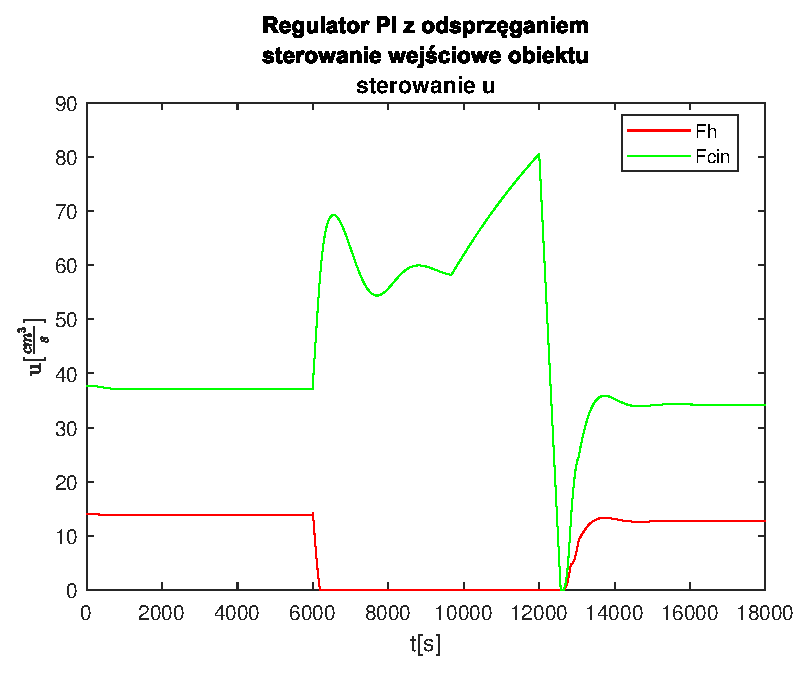
\includegraphics[width=1\linewidth]{img/PI/decoupler/noDisturbance/PIDecouplerControl1Linfalse.eps}
      \caption{}
      \label{fig:fig:PIDecoupler1Linfalse3}
   \end{subfigure}
       
   \begin{subfigure}[b]{0.4\textwidth}
      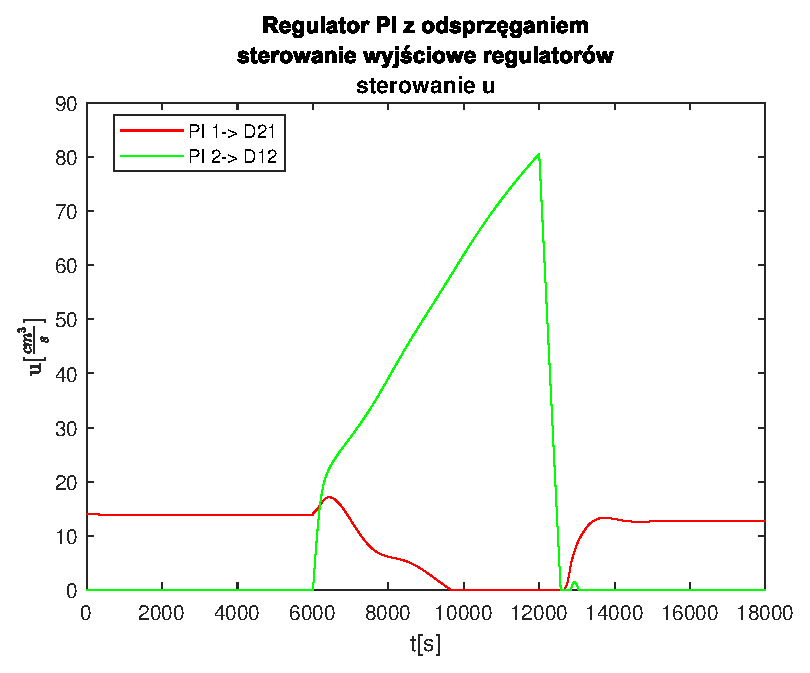
\includegraphics[width=1\linewidth]{img/PI/decoupler/noDisturbance/PIDecouplerControlD1Linfalse.eps}
      \caption{}
      \label{fig:fig:PIDecoupler1Linfalse4}
   \end{subfigure}
       
   \caption{Wykresy dla regulatora PI z odsprzeganiem.}
   \label{fig:PIDecoupler1Linfalse}
\end{figure}
           
\begin{figure}[h!]
   \centering
   \begin{subfigure}[b]{0.4\textwidth}
      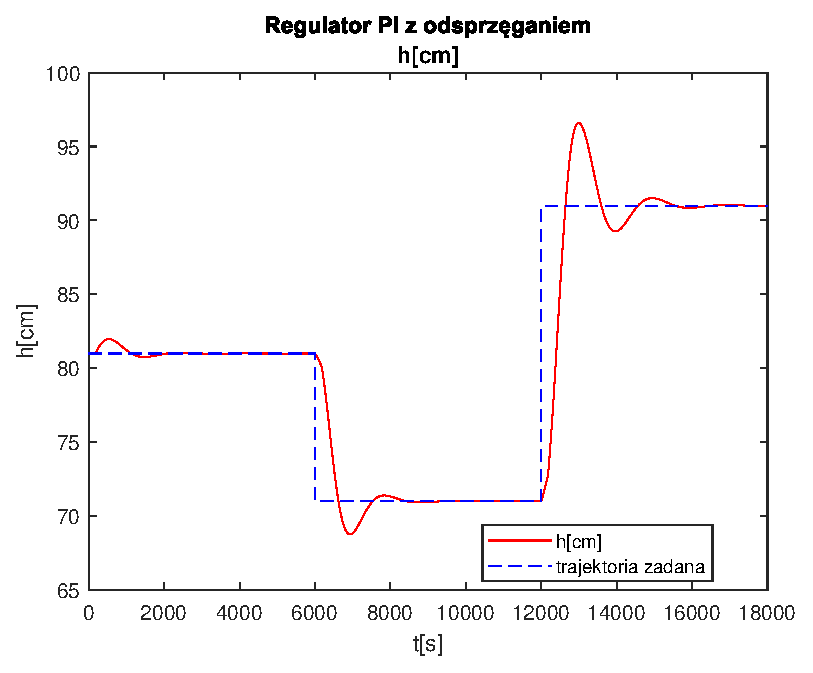
\includegraphics[width=1\linewidth]{img/PI/decoupler/noDisturbance/PIDecouplerH2Linfalse.eps}
      \caption{}
      \label{fig:fig:PIDecoupler2Linfalse1}
   \end{subfigure}
       
   \begin{subfigure}[b]{0.4\textwidth}
      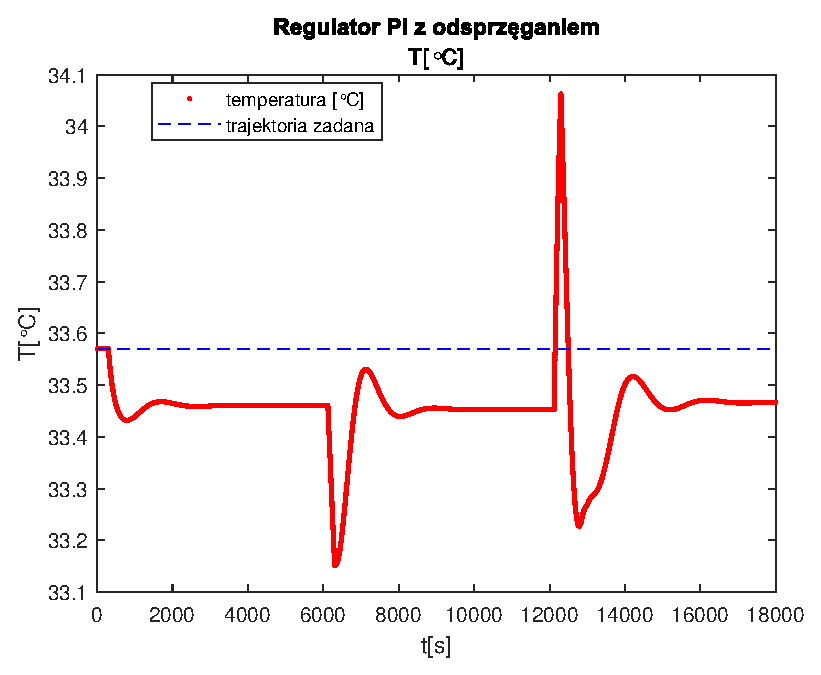
\includegraphics[width=1\linewidth]{img/PI/decoupler/noDisturbance/PIDecouplerT2Linfalse.eps}
      \caption{}
      \label{fig:fig:PIDecoupler2Linfalse2}
   \end{subfigure}
       
   \begin{subfigure}[b]{0.4\textwidth}
      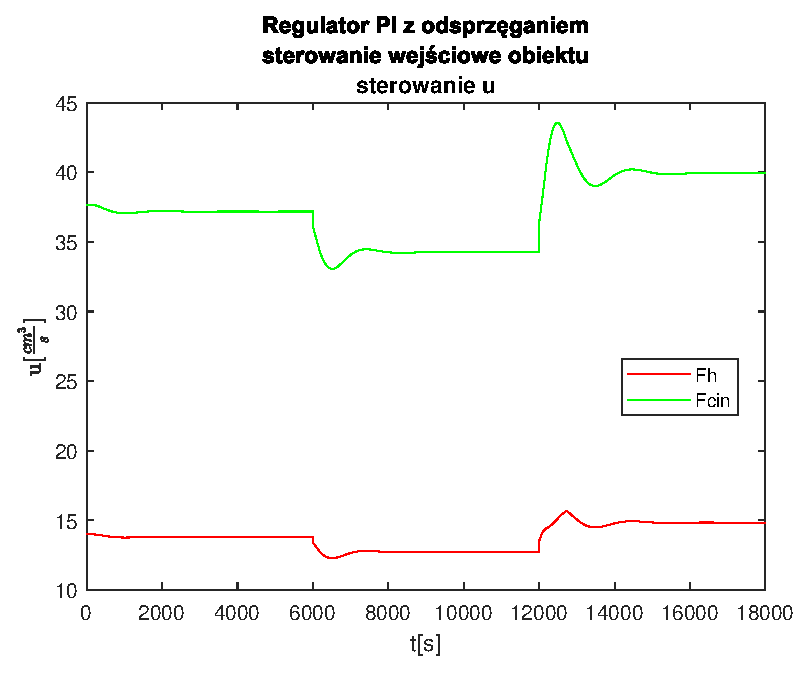
\includegraphics[width=1\linewidth]{img/PI/decoupler/noDisturbance/PIDecouplerControl2Linfalse.eps}
      \caption{}
      \label{fig:fig:PIDecoupler2Linfalse3}
   \end{subfigure}
       
   \begin{subfigure}[b]{0.4\textwidth}
      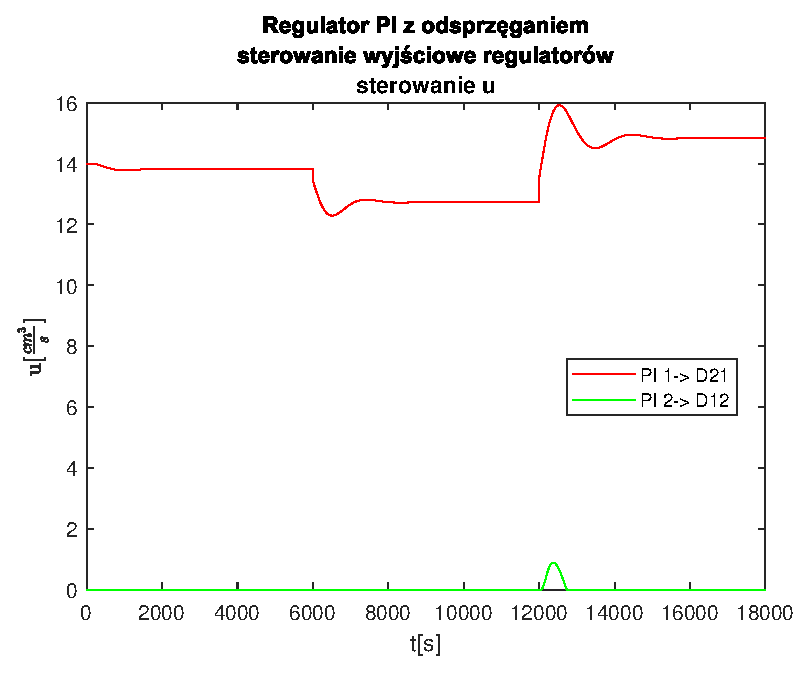
\includegraphics[width=1\linewidth]{img/PI/decoupler/noDisturbance/PIDecouplerControlD2Linfalse.eps}
      \caption{}
      \label{fig:fig:PIDecoupler2Linfalse4}
   \end{subfigure}
       
   \caption{Wykresy dla regulatora PI z odsprzeganiem.}
   \label{fig:PIDecoupler2Linfalse}
\end{figure}
           
\begin{figure}[h!]
   \centering
   \begin{subfigure}[b]{0.4\textwidth}
      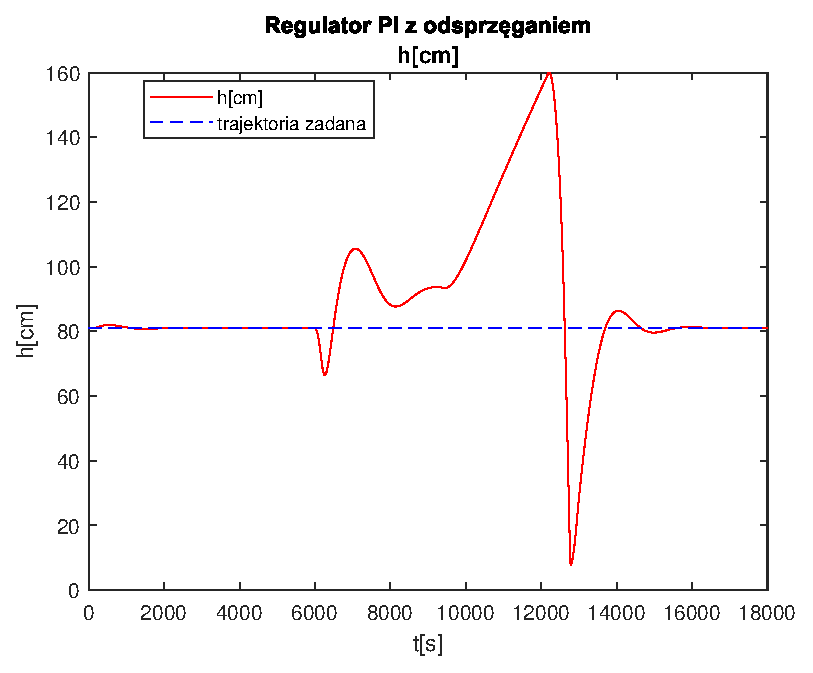
\includegraphics[width=1\linewidth]{img/PI/decoupler/noDisturbance/PIDecouplerH3Linfalse.eps}
      \caption{}
      \label{fig:fig:PIDecoupler3Linfalse1}
   \end{subfigure}
       
   \begin{subfigure}[b]{0.4\textwidth}
      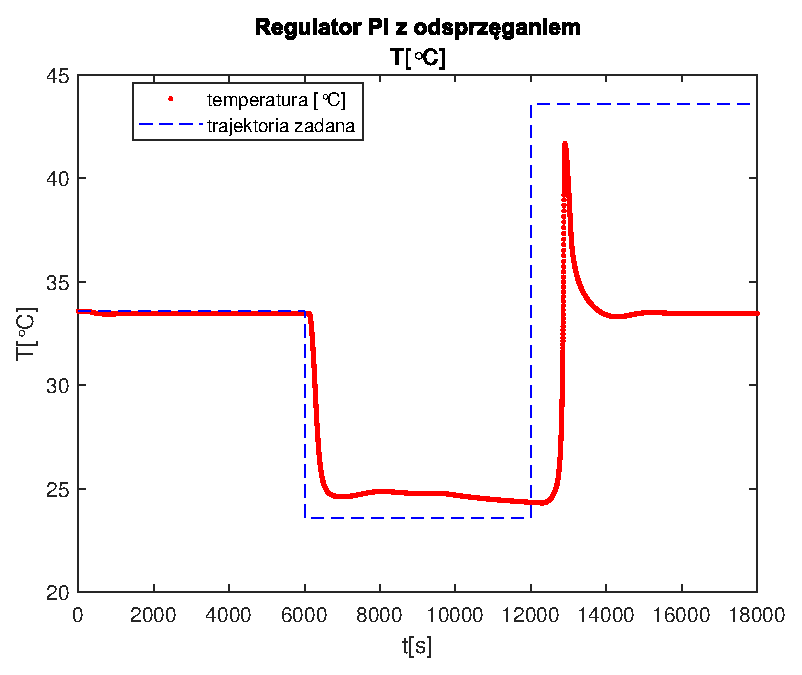
\includegraphics[width=1\linewidth]{img/PI/decoupler/noDisturbance/PIDecouplerT3Linfalse.eps}
      \caption{}
      \label{fig:fig:PIDecoupler3Linfalse2}
   \end{subfigure}
       
   \begin{subfigure}[b]{0.4\textwidth}
      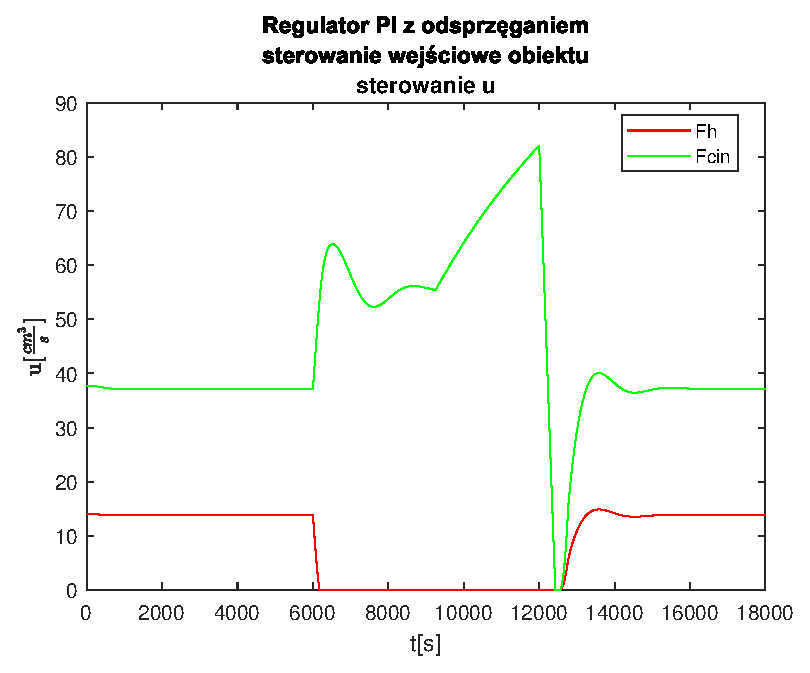
\includegraphics[width=1\linewidth]{img/PI/decoupler/noDisturbance/PIDecouplerControl3Linfalse.eps}
      \caption{}
      \label{fig:fig:PIDecoupler3Linfalse3}
   \end{subfigure}
       
   \begin{subfigure}[b]{0.4\textwidth}
      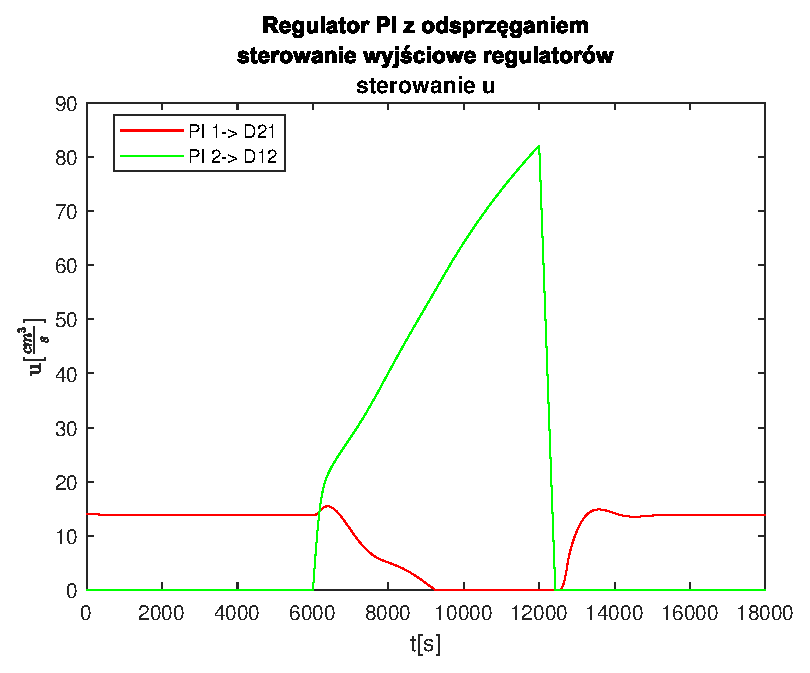
\includegraphics[width=1\linewidth]{img/PI/decoupler/noDisturbance/PIDecouplerControlD3Linfalse.eps}
      \caption{}
      \label{fig:fig:PIDecoupler3Linfalse4}
   \end{subfigure}
       
   \caption{Wykresy dla regulatora PI z odsprzeganiem.}
   \label{fig:PIDecoupler3Linfalse}
\end{figure}
           
